\documentclass[10pt,twocolumn,letterpaper]{article}

\usepackage{cvpr}
\usepackage{times}
\usepackage{epsfig}
\usepackage{graphicx}
\usepackage{amsmath}
\usepackage{amssymb}

% Include other packages here, before hyperref.

% If you comment hyperref and then uncomment it, you should delete
% egpaper.aux before re-running latex.  (Or just hit 'q' on the first latex
% run, let it finish, and you should be clear).
%\usepackage[pagebackref=true,breaklinks=true,letterpaper=true,colorlinks,bookmarks=false]{hyperref}

\cvprfinalcopy % *** Uncomment this line for the final submission

\def\cvprPaperID{} % *** Enter the 3DV Paper ID here
\def\httilde{\mbox{\tt\raisebox{-.5ex}{\symbol{126}}}}

% Pages are numbered in submission mode, and unnumbered in camera-ready
%\ifcvprfinal\pagestyle{empty}\fi
\setcounter{page}{1}
\begin{document}

%%%%%%%%% TITLE
\title{Structure from Motion with RGB-D}

\author{Seonwook Park \\
ETH Zurich \\
{\tt\small spark@student.ethz.ch}
% For a paper whose authors are all at the same institution,
% omit the following lines up until the closing ``}''.
% Additional authors and addresses can be added with ``\and'',
% just like the second author.
% To save space, use either the email address or home page, not both
\and
Yifan Wang \\
ETH Zurich \\
{\tt\small yifan.wang@student.ethz.ch}
}

\maketitle
%\thispagestyle{empty}

%%%%%%%%% ABSTRACT
\begin{abstract}
   The ABSTRACT is to be in fully-justified italicized text, at the top
   of the left-hand column, below the author and affiliation
   information. Use the word ``Abstract'' as the title, in 12-point
   Times, boldface type, centered relative to the column, initially
   capitalized. The abstract is to be in 10-point, single-spaced type.
   Leave two blank lines after the Abstract, then begin the main text.
   Look at previous 3DIMPVT/3DIM/3DPVT abstracts to get a feel for style and length.
\end{abstract}

%%%%%%%%% BODY TEXT
\section{Introduction}

Structure from Motion (SfM) concerns the recreation of a real environment
through the inferring of motion from images. (1) First, a 3D object or
environment is imaged from multiple different perspectives. (2) In each image,
it is possible to find keypoints via feature detection algorithms such as SIFT
and SURF, and calculate descriptors with which correspondences can be found in
other images. (3) After finding corresponding pairs, the relative pose of each
camera can be inferred in various ways.

With early implementations of SfM, keypoints are projected into 3D space and
optimisation algorithms such as RANSAC and Levenberg-Marquardt are used to find
the homography or perspective transformation between two image planes. With the
advent of low-cost commercial depth sensing cameras, it is now possible to
incorporate depth information in hopes to improve or speed this procedure up. An
example is the Microsoft Kinect, which casts and reads an infra-red pattern
which is used to calculate depth values per pixel imaged \cite{zhang2012microsoft}.

For problems of corresponding 2D points (image plane) and 3D points (using depth
values), one can use PnP or Perspective-n-Point algorithms \cite{d2013p3p}. A P3P
algorithm uses a minimum of 3 data points to infer the relative pose between a
pair of cameras. There are optimised PnP algorithms available, which when
coupled with RANSAC can discard outliers and estimate relative camera pose
accurately \cite{lepetit2009epnp}.

Once an initial estimate for relative camera pose is made, this can be optimised
via bundle adjustment, an optimisation step operated on sparse keypoints from
the perspective of all cameras. To do so, (4) pairwise camera pose estimates
need to be transformed into a single coordinate system. This is achieved through
the construction of a minimum spanning tree with cameras as nodes and the
existence of corresponding pairs as edges. When camera pose estimates are
relative to a single coordinate system, it is possible to project keypoints into
the coordinate system from the perspective of each camera. Minimising this
reprojection is the (5) bundle adjustment step.

A final model can be constructed by projecting all known data into 3D space
using final camera pose estimates. In such a way a dense 3D reconstruction is
possible.

This study concerns the use of depth data in hopes to improve the accuracy of
the final 3D reconstruction output.


%-------------------------------------------------------------------------

\section{Theory}

%-------------------------------------------------------------------------

\section{Methodology}

As outlined in the previous sections, our structure from motion pipeline is
composed of 5 main steps listed below.

\begin{enumerate}
\item Data acquisition
\item Feature detection and matching
\item Pairwise camera pose estimation
\item Transform to global coordinate system
\item Bundle adjustment
\end{enumerate}

It is important to note that the acquired images in this case is RGB-D and is
acquired using a Microsoft Kinect (first generation).

The pipeline is implemented in C++. Third party libraries used include OpenCV
3.0, Ceres Solver and PCL 1.8.

%-------------------------------------------------------------------------

\subsection{Data acquisition}

OpenNI and OpenCV are used to acquire RGB images and depth maps from a Kinect.
The two output images are stored with the same timestamps. The code used for
this step is provided by our supervisor, Bernhard Zeisl.

It is worth noting that the Kinect returns depth in mm in range $[0, 10000]$
which is stored as a 16-bit unsigned integer. Camera parameters are taken from
\cite{smisek20133d} and used in methods in the following steps.

While acquiring data, we attempt to find areas with sufficient potential
features and try to maximise the overlap between each shot to retain enough
correspondences.

\begin{figure}[t]
\begin{center}
   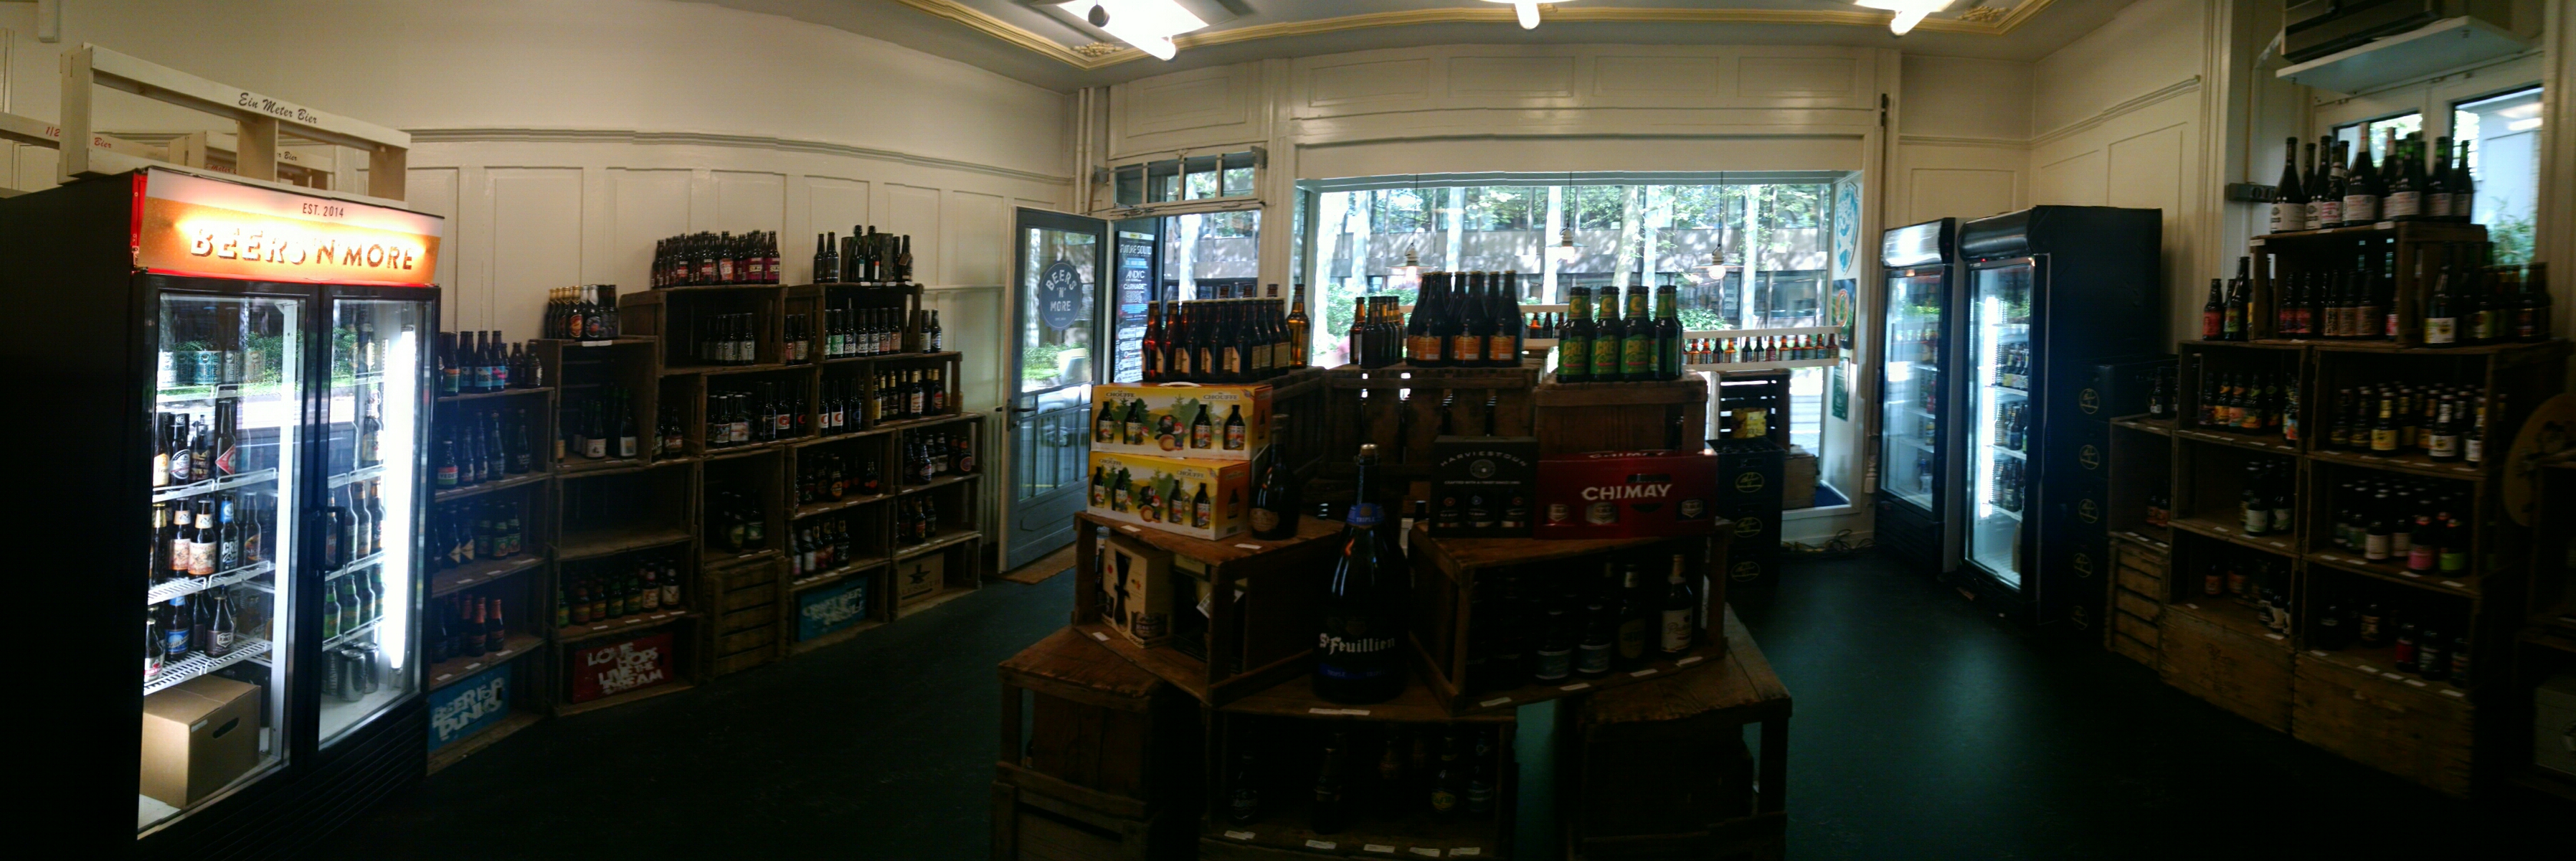
\includegraphics[width=1.0\linewidth]{figures/BeersNMore_panorama.jpg}
\end{center}
\caption{Panorama of BeersNMore interior, displaying a high number of features}
\label{fig:panorama}
\end{figure}

This resulted in the BeersNMore dataset, taken at a craft beer shop on
Universit\"atstrasse. The interior of the shop (as seen in figure \ref{fig:panorama}) exhibits
numerous unique and repeating features in the form of labelled beer bottles
boxes, and crates. The dataset consists of 229 RGB and depth images.



%-------------------------------------------------------------------------

\subsection{Feature detection and matching}

For each given RGB image, SIFT features are found, and 128-dimensional are
descriptors calculated. Standard OpenCV parameters are used for this step.

A matching algorithm is then run between all potential image pairs. This is
an $\mathcal{O}(n^2)$ operation. The matcher compares the distance between
descriptors and finds those with minimum distance. This produces numerous
incorrect matches, often visible by the violation of epipolar geometry.

The matching is therefore performed in a bi-directional manner, both from image
$i$ to $j$, and $j$ to $i$. This results in a better sample of matches. RANSAC
can be used in the camera registration step to further eliminate outliers.



%-------------------------------------------------------------------------

\subsection{Pairwise camera pose estimation}

The previous step yields a list of image pairs which have matching features.
The discovered features from image $i$ can then be projected into 3D space
using its depth map values, and reprojected into image $j$. The minimisation
of this error is carried out using OpenCV's EPnP solver.

The mentioned solver also identifies outlier matches via RANSAC. Only inliers
are retained to improve any further optimisations. To ensure that only good
image pairs are retained, we also filter these image pairs based on an absolute
minimum number of inliers of 30. If two images have less then 30 feature matches
which are inliers in the registration process, it is assumed that the image pair
is not good enough for subsequent steps.

Similar to the feature matching step, the PnP solver is run in both directions,
projecting 3D points from image $i$ into image $j$, and projecting 3D points
from image $j$ into image $i$. This allows for two things, (1) the averaging of
pose estimates to improve accuracy and (2) reduction of bad matches where
relative rotation vectors do not add up to 0.

The final output from this step is a list of camera pairs which are deemed to
have good matching features, and associated pairwise camera pose estimates.


%-------------------------------------------------------------------------

\subsection{Transform to global coordinate system}

The final goal of this SfM pipeline is to combine the data from all images
acquired. To do so, previously acquired pairwise camera pose estimates must
be transformed into a single coordinate frame.

\begin{figure}[t]
\begin{center}
   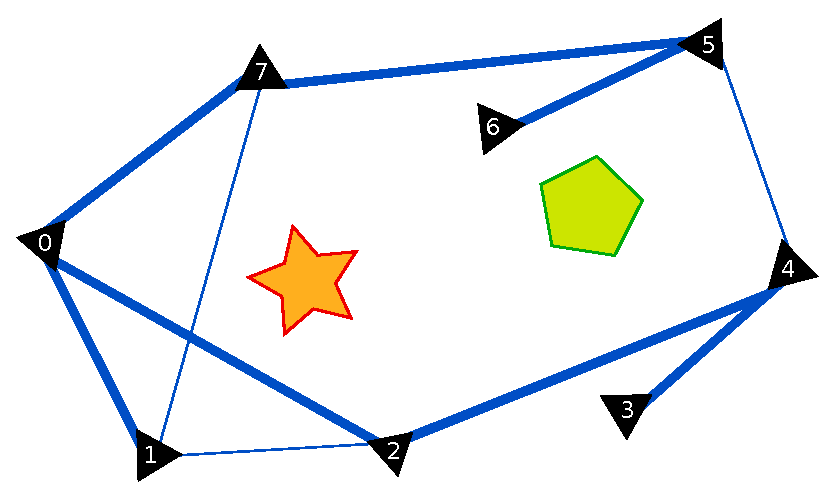
\includegraphics[width=0.9\linewidth]{figures/spanning_tree.eps}
\end{center}
\caption{An example of a minimum spanning tree in terms of this pipeline}
\label{fig:spanning}
\end{figure}

The 0th camera is selected to be the reference coordinate frame. A breadth-first
algorithm is used to construct a minimum spanning tree with cameras as nodes and
the existence of camera pose estimate as edges (whether an image pair exists).
The spanning tree can be walked to calculate camera pose estimates relative to
the 0th camera.

\begin{figure}[t]
\begin{center}
   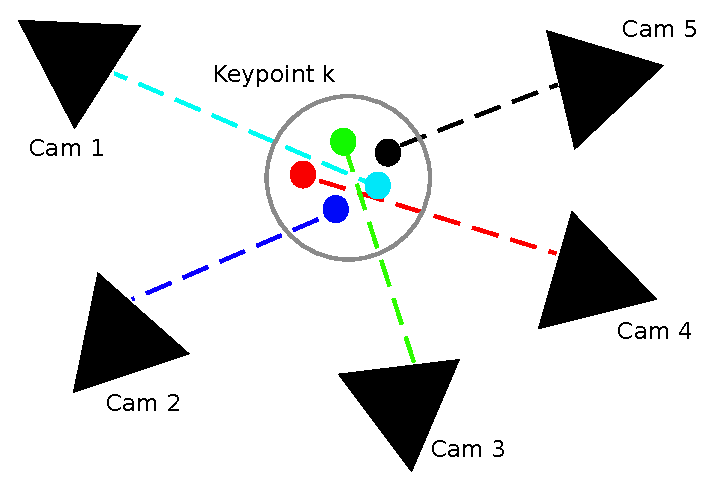
\includegraphics[width=0.9\linewidth]{figures/clusters.eps}
\end{center}
\caption{An example of a cluster of keypoint pose estimations}
\label{fig:spanning}
\end{figure}

The outcome of this step needs to be a cloud of keypoints and camera pose
estimates in global coordinate frame. However, each keypoint is observed by a
minimum of two cameras, resulting in a cluster of keypoint coordinate estimates.
The centre of mass (CoM) of this cluster is calculated by averaging the
coordinate estimations. This results in a single keypoint coordinate estimate,
and consequently an initial point cloud of sparse features.

%-------------------------------------------------------------------------

\subsection{Bundle adjustment}


%-------------------------------------------------------------------------

\section{Results and discussion}


%-------------------------------------------------------------------------

\section{Conclusion}


%-------------------------------------------------------------------------
\clearpage
\clearpage

\subsection{Mathematics}

Please number all of your sections and displayed equations.  It is
important for readers to be able to refer to any particular equation.  Just
because you didn't refer to it in the text doesn't mean some future reader
might not need to refer to it.  It is cumbersome to have to use
circumlocutions like ``the equation second from the top of page 3 column
1''.  (Note that the ruler will not be present in the final copy, so is not
an alternative to equation numbers).  All authors will benefit from reading
Mermin's description of how to write mathematics.%: \url{http://www.cvpr.org/doc/mermin.pdf}.


\subsection{Blind review}

Many authors misunderstand the concept of anonymizing for blind
review.  Blind review does not mean that one must remove
citations to one's own work---in fact it is often impossible to
review a paper unless the previous citations are known and
available.

Blind review means that you do not use the words ``my'' or ``our''
when citing previous work.  That is all.  (But see below for
techreports)

Saying ``this builds on the work of Lucy Smith [1]'' does not say
that you are Lucy Smith, it says that you are building on her
work.  If you are Smith and Jones, do not say ``as we show in
[7]'', say ``as Smith and Jones show in [7]'' and at the end of the
paper, include reference 7 as you would any other cited work.

An example of a bad paper just asking to be rejected:
\begin{quote}
\begin{center}
    An analysis of the frobnicatable foo filter.
\end{center}

   In this paper we present a performance analysis of our
   previous paper [1], and show it to be inferior to all
   previously known methods.  Why the previous paper was
   accepted without this analysis is beyond me.

   [1] Removed for blind review
\end{quote}


An example of an acceptable paper:

\begin{quote}
\begin{center}
     An analysis of the frobnicatable foo filter.
\end{center}

   In this paper we present a performance analysis of the
   paper of Smith \etal [1], and show it to be inferior to
   all previously known methods.  Why the previous paper
   was accepted without this analysis is beyond me.

   [1] Smith, L and Jones, C. ``The frobnicatable foo
   filter, a fundamental contribution to human knowledge''.
   Nature 381(12), 1-213.
\end{quote}

If you are making a submission to another conference at the same time,
which covers similar or overlapping material, you may need to refer to that
submission in order to explain the differences, just as you would if you
had previously published related work.  In such cases, include the
anonymized parallel submission~\cite{Authors12} as additional material and
cite it as
\begin{quote}
[1] Authors. ``The frobnicatable foo filter'', F\&G 2012 Submission ID 324,
Supplied as additional material {\tt fg324.pdf}.
\end{quote}

Finally, you may feel you need to tell the reader that more details can be
found elsewhere, and refer them to a technical report.  For conference
submissions, the paper must stand on its own, and not {\em require} the
reviewer to go to a techreport for further details.  Thus, you may say in
the body of the paper ``further details may be found
in~\cite{Authors12b}''.  Then submit the techreport as additional material.
Again, you may not assume the reviewers will read this material.

Sometimes your paper is about a problem which you tested using a tool which
is widely known to be restricted to a single institution.  For example,
let's say it's 1969, you have solved a key problem on the Apollo lander,
and you believe that the 3DV70 audience would like to hear about your
solution.  The work is a development of your celebrated 1968 paper entitled
``Zero-g frobnication: How being the only people in the world with access to
the Apollo lander source code makes us a wow at parties'', by Zeus \etal.

You can handle this paper like any other.  Don't write ``We show how to
improve our previous work [Anonymous, 1968].  This time we tested the
algorithm on a lunar lander [name of lander removed for blind review]''.
That would be silly, and would immediately identify the authors. Instead
write the following:
\begin{quotation}
\noindent
   We describe a system for zero-g frobnication.  This
   system is new because it handles the following cases:
   A, B.  Previous systems [Zeus et al. 1968] didn't
   handle case B properly.  Ours handles it by including
   a foo term in the bar integral.

   ...

   The proposed system was integrated with the Apollo
   lunar lander, and went all the way to the moon, don't
   you know.  It displayed the following behaviours
   which show how well we solved cases A and B: ...
\end{quotation}
As you can see, the above text follows standard scientific convention,
reads better than the first version, and does not explicitly name you as
the authors.  A reviewer might think it likely that the new paper was
written by Zeus \etal, but cannot make any decision based on that guess.
He or she would have to be sure that no other authors could have been
contracted to solve problem B.

FAQ: Are acknowledgements OK?  No.  Leave them for the final copy.


\begin{figure}[t]
\begin{center}
\fbox{\rule{0pt}{2in} \rule{0.9\linewidth}{0pt}}
   %\includegraphics[width=0.8\linewidth]{egfigure.eps}
\end{center}
   \caption{Example of caption.  It is set in Roman so that mathematics
   (always set in Roman: $B \sin A = A \sin B$) may be included without an
   ugly clash.}
\label{fig:long}
\label{fig:onecol}
\end{figure}

\subsection{Miscellaneous}

\noindent
Compare the following:\\
\begin{tabular}{ll}
 \verb'$conf_a$' &  $conf_a$ \\
 \verb'$\mathit{conf}_a$' & $\mathit{conf}_a$
\end{tabular}\\
See The \TeX book, p165.

The space after \eg, meaning ``for example'', should not be a
sentence-ending space. So \eg is correct, {\em e.g.} is not.  The provided
\verb'\eg' macro takes care of this.

When citing a multi-author paper, you may save space by using ``et alia'',
shortened to ``\etal'' (not ``{\em et.\ al.}'' as ``{\em et}'' is a complete word.)
However, use it only when there are three or more authors.  Thus, the
following is correct: ``
   Frobnication has been trendy lately.
   It was introduced by Alpher~\cite{Alpher02}, and subsequently developed by
   Alpher and Fotheringham-Smythe~\cite{Alpher03}, and Alpher \etal~\cite{Alpher04}.''

This is incorrect: ``... subsequently developed by Alpher \etal~\cite{Alpher03} ...''
because reference~\cite{Alpher03} has just two authors.  If you use the
\verb'\etal' macro provided, then you need not worry about double periods
when used at the end of a sentence as in Alpher \etal.

For this citation style, keep multiple citations in numerical (not
chronological) order, so prefer \cite{Alpher03,Alpher02,Authors12} to
\cite{Alpher02,Alpher03,Authors12}.


\begin{figure*}
\begin{center}
\fbox{\rule{0pt}{2in} \rule{.9\linewidth}{0pt}}
\end{center}
   \caption{Example of a short caption, which should be centered.}
\label{fig:short}
\end{figure*}

%------------------------------------------------------------------------
\section{Formatting your paper}

All text must be in a two-column format. The total allowable width of the
text area is $6\frac78$ inches (17.5 cm) wide by $8\frac78$ inches (22.54
cm) high. Columns are to be $3\frac14$ inches (8.25 cm) wide, with a
$\frac{5}{16}$ inch (0.8 cm) space between them. The main title (on the
first page) should begin 1.0 inch (2.54 cm) from the top edge of the
page. The second and following pages should begin 1.0 inch (2.54 cm) from
the top edge. On all pages, the bottom margin should be 1-1/8 inches (2.86
cm) from the bottom edge of the page for $8.5 \times 11$-inch paper; for A4
paper, approximately 1-5/8 inches (4.13 cm) from the bottom edge of the
page.

%-------------------------------------------------------------------------
\subsection{Margins and page numbering}

All printed material, including text, illustrations, and charts, must be kept
within a print area 6-7/8 inches (17.5 cm) wide by 8-7/8 inches (22.54 cm)
high.  Page numbers should be in footer with page numbers, centered and .75
inches from the bottom of the page and make it start at the correct page
number rather than the 4321 in the example.  To do this fine the line (around
line 23)
\begin{verbatim}
%\ifcvprfinal\pagestyle{empty}\fi
\setcounter{page}{4321}
\end{verbatim}
where the number 4321 is your assigned starting page.

Make sure the first page is numbered by commenting out the first page being
empty on line 46
\begin{verbatim}
%\thispagestyle{empty}
\end{verbatim}


%-------------------------------------------------------------------------
\subsection{Type-style and fonts}

Wherever Times is specified, Times Roman may also be used. If neither is
available on your word processor, please use the font closest in
appearance to Times to which you have access.

MAIN TITLE. Center the title 1-3/8 inches (3.49 cm) from the top edge of
the first page. The title should be in Times 14-point, boldface type.
Capitalize the first letter of nouns, pronouns, verbs, adjectives, and
adverbs; do not capitalize articles, coordinate conjunctions, or
prepositions (unless the title begins with such a word). Leave two blank
lines after the title.

AUTHOR NAME(s) and AFFILIATION(s) are to be centered beneath the title
and printed in Times 12-point, non-boldface type. This information is to
be followed by two blank lines.

The ABSTRACT and MAIN TEXT are to be in a two-column format.

MAIN TEXT. Type main text in 10-point Times, single-spaced. Do NOT use
double-spacing. All paragraphs should be indented 1 pica (approx. 1/6
inch or 0.422 cm). Make sure your text is fully justified---that is,
flush left and flush right. Please do not place any additional blank
lines between paragraphs.

Figure and table captions should be 9-point Roman type as in
Figures~\ref{fig:onecol} and~\ref{fig:short}.  Short captions should be centred.

\noindent Callouts should be 9-point Helvetica, non-boldface type.
Initially capitalize only the first word of section titles and first-,
second-, and third-order headings.

FIRST-ORDER HEADINGS. (For example, {\large \bf 1. Introduction})
should be Times 12-point boldface, initially capitalized, flush left,
with one blank line before.

SECOND-ORDER HEADINGS. (For example, { \bf 1.1. Database elements})
should be Times 11-point boldface, initially capitalized, flush left,
with one blank line before, and one after. If you require a third-order
heading (we discourage it), use 10-point Times, boldface, initially
capitalized, flush left, preceded by one blank line, followed by a period
and your text on the same line.

%-------------------------------------------------------------------------
\subsection{Footnotes}

Please use footnotes\footnote {This is what a footnote looks like.  It
often distracts the reader from the main flow of the argument.} sparingly.
Indeed, try to avoid footnotes altogether and include necessary peripheral
observations in
the text (within parentheses, if you prefer, as in this sentence).  If you
wish to use a footnote, place it at the bottom of the column on the page on
which it is referenced. Use Times 8-point type, single-spaced.


%-------------------------------------------------------------------------
\subsection{References}

List and number all bibliographical references in 9-point Times,
single-spaced, at the end of your paper. When referenced in the text,
enclose the citation number in square brackets, for
example~\cite{Authors12}.  Where appropriate, include the name(s) of
editors of referenced books.

\begin{table}
\begin{center}
\begin{tabular}{|l|c|}
\hline
Method & Frobnability \\
\hline\hline
Theirs & Frumpy \\
Yours & Frobbly \\
Ours & Makes one's heart Frob\\
\hline
\end{tabular}
\end{center}
\caption{Results.   Ours is better.}
\end{table}

%-------------------------------------------------------------------------
\subsection{Illustrations, graphs, and photographs}

All graphics should be centered.  Please ensure that any point you wish to
make is resolvable in a printed copy of the paper.  Resize fonts in figures
to match the font in the body text, and choose line widths which render
effectively in print.  Many readers (and reviewers), even of an electronic
copy, will choose to print your paper in order to read it.  You cannot
insist that they do otherwise, and therefore must not assume that they can
zoom in to see tiny details on a graphic.

When placing figures in \LaTeX, it's almost always best to use
\verb+\includegraphics+, and to specify the  figure width as a multiple of
the line width as in the example below
{\small\begin{verbatim}
   \usepackage[dvips]{graphicx} ...
   \includegraphics[width=0.8\linewidth]
                   {myfile.eps}
\end{verbatim}
}


%-------------------------------------------------------------------------
\subsection{Color}

Color is valuable, and will be visible to readers of the electronic copy.
However ensure that, when printed on a monochrome printer, no important
information is lost by the conversion to grayscale.

%------------------------------------------------------------------------
\section{Final copy}

You must include your signed IEEE copyright release form when you submit
your finished paper. We MUST have this form before your paper can be
published in the proceedings.


{\small
\bibliographystyle{ieee}
\bibliography{egbib}
}

\end{document}
